\subsection{Numerical Experiments}
    
    Now, we will proceed to describe the steps necessary to implement the method based on the above:
    \begin{enumerate}
    	\item Set the intervals to consider, $[0, 1]$ for physical space and $[0, t_f]$ for time with $t_f$ fixed, and give the functional $u_0$ that interacting with the initial condition $x(\xi)$ . It is also necessary to choose the values of $N, M, N_1$, and another for the parameter $\alpha$. 
    	
    	\item We proceed to calculate the points $\xi_i \in [0, 1]$ for $i = 0, 1, \dots, p$ with $p$ positive entire as
    	\begin{align*}
    		\xi_i = \xi_0 + i \Delta \xi, \hspace{2mm} i = 0, 1, \dots, p
    	\end{align*}
    	and to obtain the points $t_j \in [t_0, t_f]$, we define the sequence $j = 0, 1, \dots, T$, for some positive entire $T$, and calculate the following
    	\begin{align*}
    		t_j = t_0 + j \Delta t, \hspace{2mm} \Delta t = \frac{t_f}{T} 
    	\end{align*}
    	
    	\item Calculate the values of $\mathcal{J}^{N, M}$ to obtain the matrix $\bar{C}_{n, m}$. Setting the values $\lambda_i$ to proceed with the calculation of the eigenvalues $\eta_i$ and their respective eigenvectors $V_i$ of the matrix $A$.
    	
    	\item Using the functional $u_0$ to calculate the constants $c_k$ for each $k = 1, \dots, M$, and then obtain the system solution given by (\ref{solution_finite_system}).
    	
    	\item Finally, the approximation obtained is evaluated using the equation given by
    	\begin{align*}
    		u_M(x, t) = \displaystyle \sum_{k=1}^{M} u_k (t) H_k (x).
    	\end{align*}
    \end{enumerate}
    
    The following simulations that will be shown were performed using a discretization of $2048$ points in the spatial variable $\xi$ over the interval $[0, 1]$, and $1024$ points in the variable time $t$ over the interval $[0, 10]$. In addition, the values of the parameters $N = 5$, $M = 11$, and $\alpha = 1.0 \times 10^{-2}$ were considered. With this information, the solutions obtained were calculated using the following initial condition and its truncated Chebysheb expansion given by
    \begin{align*}
    	x(\xi) = \sin(\pi \xi), \hspace{3mm} y(\xi) = \displaystyle \sum^{N}_{k=0} c_k T_k (\xi),
    \end{align*}
    
    This numerical experiment consists of illustrating an interesting result given in \cite{Delgado2019}, which tells us that the solutions obtained from two close initial conditions also remain close. This behavior allows characterizing what is known as the stability of the approximation, and it is described by means of continuity with respect to the initial conditions of the numerical approximations of the equation (\ref{kolmogorov}). \\
    
    To understand this better, let us denote by $\Psi^{x}_t$ the solution of (\ref{kolmogorov}) obtained by
    \begin{align*}
    	u(x, t) = \mathbb{E} \left[ \varphi (X^x_t) \right]. 
    \end{align*}
    where $\varphi: \mathcal{H} \rightarrow \mathbb{R}$ is Lipschitz and $X^x_t$ is the solution to (\ref{stochastic_equation}) with initial conditions $X_0 = x \in \mathcal{H}$. So, as before, its expansion is given by
    \begin{align*}
    	\Psi^{x}_t = \displaystyle \sum _{n \in \mathcal{J}} u_n (t) H_n (x), \hspace{2mm} x \in \mathcal{H}, \hspace{2mm} t \in [0, T].
    \end{align*}
    
    Therefore, following our reference, the above is summarized as follows: Given two different initial conditions $x, y \in \mathcal{H}$, then we have the following estimate
	\begin{align*}
		\| \Psi^x_t - \Psi^y_t \|^2_{\left( L^2 (\mathcal{H}, \mu)\right)^2} \leq \exp(Ct) \displaystyle \int_{\mathcal{H} \times \mathcal{H}} \|x - y \|^2_{\mathcal{H}} \mu (dx) \mu (dy) + f(t) \|x - y\|_{\mathcal{H}},
	\end{align*}
	for some $C$ finite and $f(t)$ is given by
	\begin{align*}
		f(t) = \displaystyle \sum_{n \in J} \left[u^y_n (t)\right]^2 + \int_{\mathcal{H}} \mathbb{E}^2 \left[\varphi (X^y_t)\right] \mu (dy).
	\end{align*}	
	
	From the above, we can see that if $ \| x - y \|_{\mathcal{H}} \leq \delta$, so we have to $\| \Psi^x_t - \Psi^y_t \| \leq G (t) \delta$. As we have already mentioned, this continuity defines a type of stability for approximations, which is of utmost importance in this field since characterizations of this type are still under construction and are essential for the analysis of a numerical method. \\
	
	This behavior is shown in the following figures, which were obtained using codes that were created following the previous steps, and which can be found in \url{https://github.com/alanmatzumiya/Paper.git}. In figure \ref{IC_Cheb} it shows us the two initial conditions for which the equation (\ref{kolmogorov}) will be solved by associating it with (\ref{burgers_stochastic}), and in figure \ref{Stochastic_Solutions} we can see that the solutions keep the distance. Finally, the figure \ref{Continuity} shows the distances for each instant of time $t$, showing that they are actually getting closer as time passes.
	
\newpage
	\begin{figure}[H]	
		\centering	
		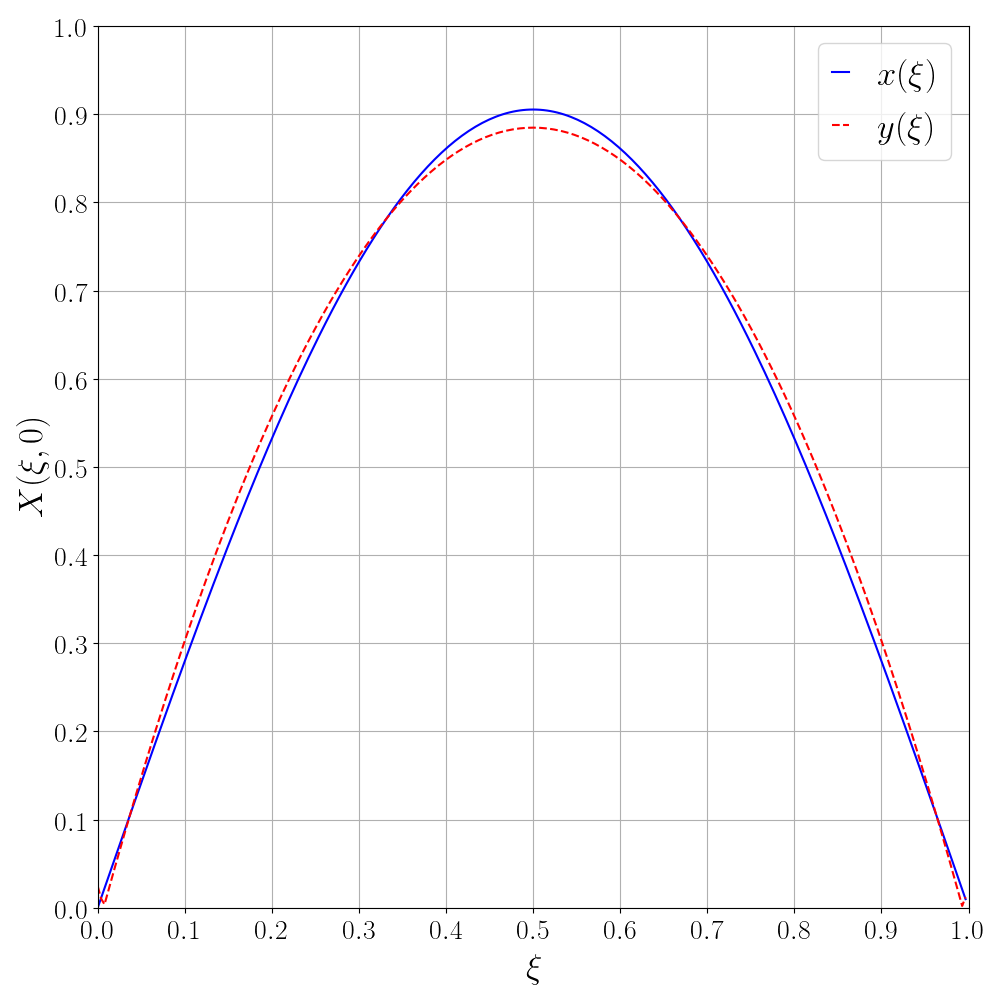
\includegraphics[width=.55\textwidth]{burgers_equation/stochastic/numerical_experiments/figures/IC.png}
		\caption{Initial condition for (\ref{burgers_stochastic2}) and its approximation.}
		\label{IC_Cheb}	
		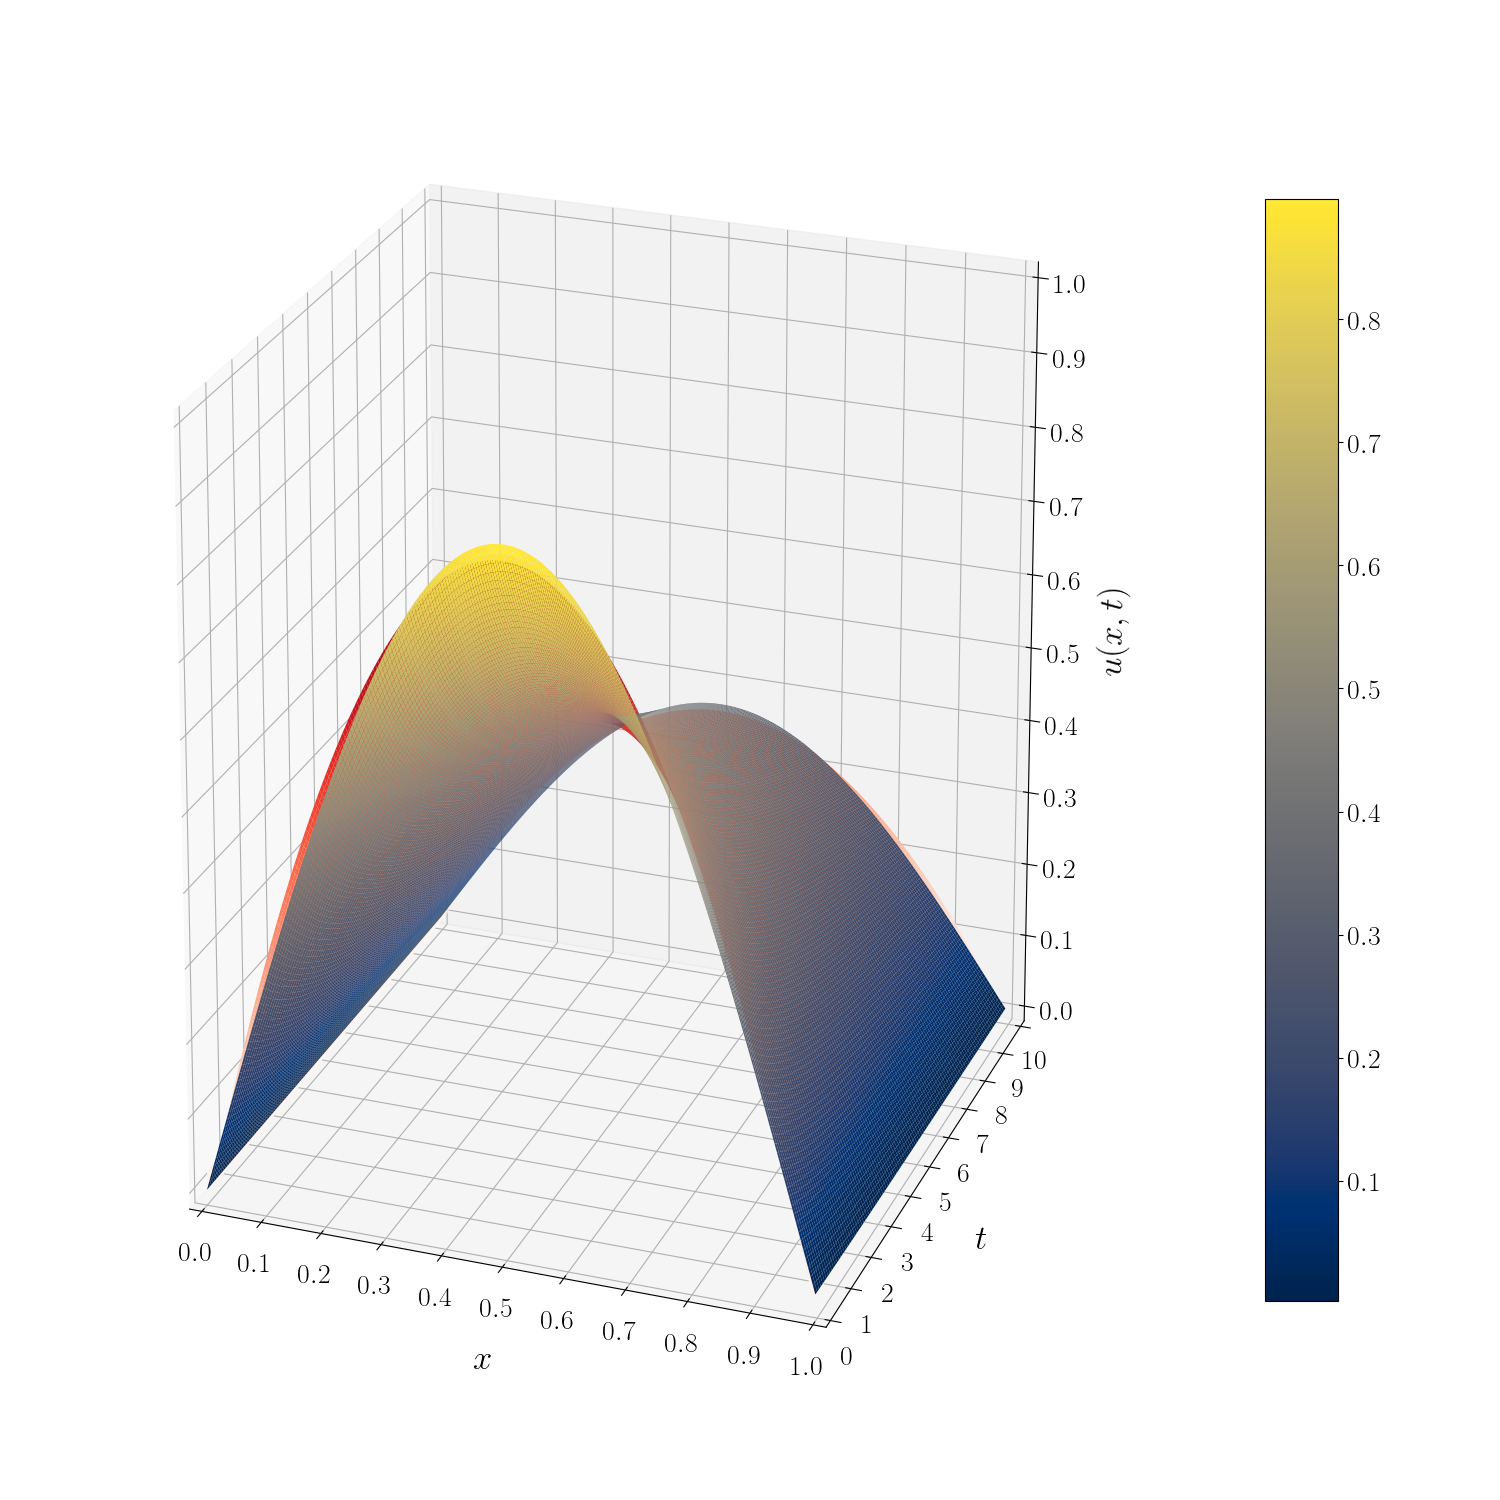
\includegraphics[width=.9\textwidth]{burgers_equation/stochastic/numerical_experiments/figures/Numerical_Solution_Stochastic.png}
		\caption{Numerical solutions for (\ref{burgers_stochastic2}) with initial conditions $x(\xi)$ and $y(\xi)$.}
		\label{Stochastic_Solutions}	
	\end{figure}
\newpage
	\begin{figure}[H]	
	\centering
		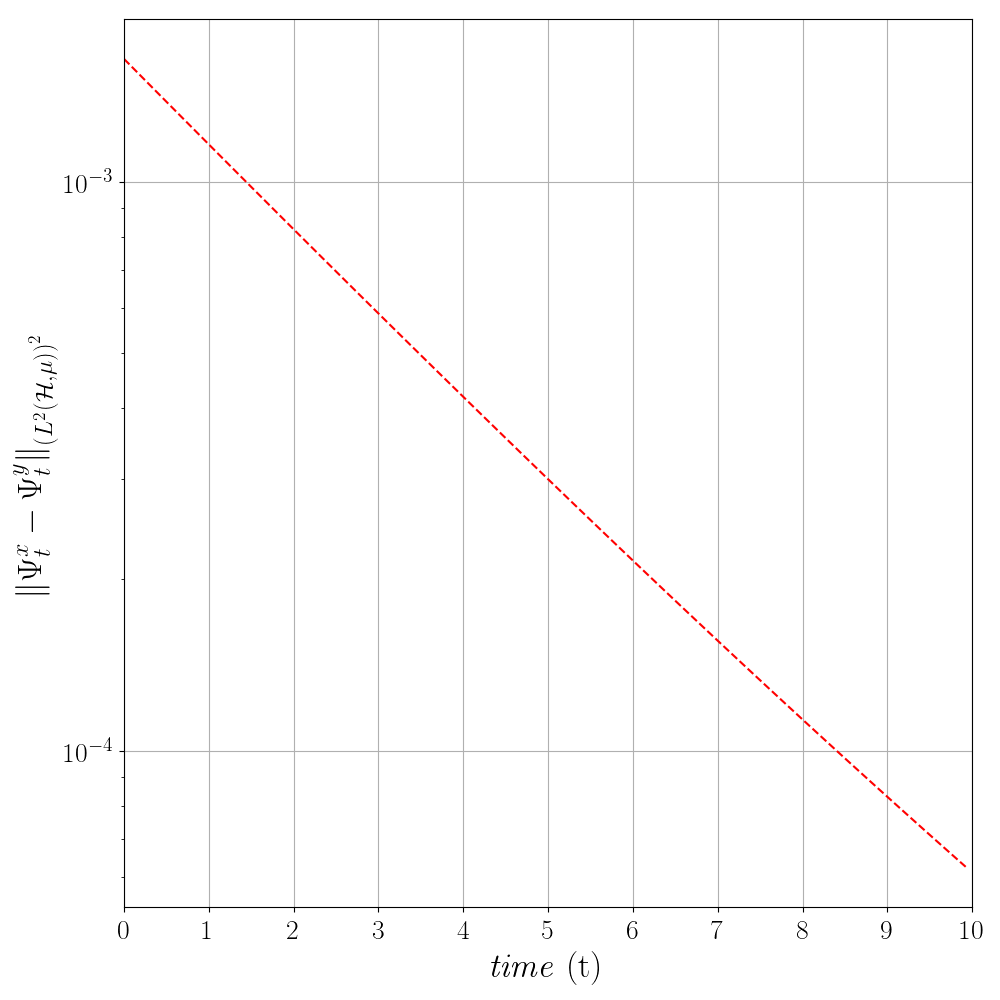
\includegraphics[width=.7\textwidth]{burgers_equation/stochastic/numerical_experiments/figures/norms.png}
		\caption{Distance between the numerical solutions for equation (\ref{burgers_stochastic2}) with initial conditions $x(\xi)$, and $y(\xi)$.}
		\label{Continuity}
	\end{figure}